\newpage
\section{LECTURE 12}

\subsection{Agenda}
\begin{itemize}
    \item LQR with Quaternions
    \item Hybrid Systems for contact
\end{itemize}

\subsection{LQR with Quaternions}
\begin{itemize}
    \item Naively linearizing a system with a quaternion state results in an uncontrollable linear system.
    \item We'll apply our quaternion differentiation tricks to LQR to make this work.
    \item Given a reference $\bar{x}_k, \bar{u}_k$ for a discret time system $f(x_k, u_k)$
    \begin{align}
        \begin{split}
            \bar{x}_{k+1} + \Delta x_{k+1} & = f(\bar{x}_k + \Delta x_k, \bar{u}_k + \Delta u_k) \\
            & \approx f(\bar{x}_k, \bar{u}_k) + A_k \Delta x_k + B_k \Delta u_k
        \end{split}
    \end{align}
    \item For the quaternion part of the state, we apply the attitude Jacobian to convert $\Delta q \to \phi \in \mathbb{R}^3$
    \begin{align}
        \begin{bmatrix}
            \Delta x_{k+1}[1:3] \\
            \phi_{k+1} \\
            \Delta x_{k+1}[8:n]
        \end{bmatrix} & = 
        \begin{bmatrix}
            I & & \\
             & G(\bar{q}_{k+1}) & \\
             & & I
        \end{bmatrix}^T A_k 
        \begin{bmatrix}
            I & & \\
             & G(\bar{q}_k) & \\
             & & I
        \end{bmatrix} + 
        \begin{bmatrix}
            I & & \\
             & G(\bar{q}_{k+1}) & \\
             & & I
        \end{bmatrix}^T B_k \Delta u_k \\
        \Delta \tilde x_{k+1} & = E(\bar{x}_{k+1}) A_k E(\bar{x}_{k}) \Delta x_k + E(\bar{x}_{k+1}) B_k \Delta u_k
    \end{align}
    \item Once we have these "reduced" Jacobians $\tilde A_k, \tilde B_k$, we compute the LQR gains as usual:
    \begin{align}
        \tilde A_k = E(\bar{x}_{k+1}) A_k E(\bar{x}_{k}), \tilde B_k = E(\bar{x}_{k+1}) B_k
    \end{align}
    \item When we run the controller, ew calculate $\Delta \tilde x$ before multiplying by K:
    \begin{align}
        \text{given } x_n, \Delta \tilde x_k & = 
        \begin{bmatrix}
            x_k[1:3] - \bar{x}_k[1:3] \\
            \phi(L(\bar{q}_k)^T q_k) \\
            x_k[8:n] - \bar{x}_k[8:n] 
        \end{bmatrix} \\
        u_k & = \bar{u}_k - K_k \Delta \tilde x_k
    \end{align}
    \item Computing delta/error rotations:
    \begin{align}
        \prescript{N}{}{Q_k}^{B_k}, \prescript{N}{}{Q_{k+1}}^{B_{k+1}} & \Rightarrow
        \prescript{B_{k+1}}{}{Q_k}^{B_k} = (\prescript{N}{}{Q_{k+1}}^{B_{k+1}}) (\prescript{N}{}{Q_k}^{B_k})^{-1} = \prescript{B_{k+1}}{}{Q_{k+1}}^N \prescript{N}{}{Q_k}^{B_k}) = Q_{k+1}^T Q_k \\
        \Delta Q = \bar{Q}^T Q & \Leftrightarrow \Delta q = \bar{q}^* * q = L(\bar{q})^T q
    \end{align}
\end{itemize}

\subsection{Example: 3D Quadrotor}

\begin{figure}
    \centering
    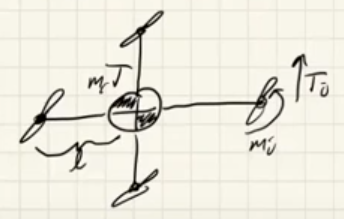
\includegraphics[width=0.4\linewidth]{L12_Images/F1.PNG}
    \caption{Quadrotor}
    \label{fig:l12f1}
\end{figure}

\begin{align}
    T_i &= K_T u_i \\
    M_i &= K_M u_i \\
    u_i &\in \mathbb{R}^4
\end{align}

\begin{itemize}
    \item State:
    \begin{align}
        x = 
        \begin{bmatrix}
            \prescript{N}{}{r} \in \mathbb{R}^3 & \text{position in N frame} \\
            q \in \mathbb{H} & \text{attitude } (B \to N)\\
            \prescript{B}{}{v} \in \mathbb{R}^3 & \text{linear velocity in B frame} \\
            \prescript{B}{}{\omega} \in \mathbb{R}^3 & \text{angular velocity in B frame} \\
        \end{bmatrix}
    \end{align}
    \item Kinematics:
    \begin{align}
        \prescript{N}{}{\dot r} & = \prescript{N}{}{v} = Q \prescript{B}{}{v} \\
        \dot q & = \frac{1}{2}q * \omega = \frac{1}{2} L(q) H ^B \omega
    \end{align}
    \item Translation Dynamics:
    \begin{align}
        m \prescript{N}{}{\dot v} & = \prescript{N}{}{F} \\
        \prescript{N}{}{v} & = Q \prescript{B}{}{v} \Rightarrow \prescript{N}{}{\dot v} = \dot Q \prescript{B}{}{v} + Q \prescript{B}{}{\dot v} = Q \hat \omega \prescript{B}{}{v} + Q \prescript{B}{}{\dot v} \\
        \Rightarrow \prescript{B}{}{\dot v} & = Q^T \prescript{N}{}{\dot v} - \prescript{B}{}{\omega} \times \prescript{B}{}{v} \\
        \Rightarrow \prescript{B}{}{\dot v} & = \frac{1}{m} \prescript{B}{}{F} - \prescript{B}{}{\omega} \times \prescript{B}{}{v} \\
        \prescript{B}{}{F} & = Q^T 
        \begin{bmatrix}
            0 \\ 0 \\ -mg
        \end{bmatrix} + 
        \begin{bmatrix}
            0 & 0 & 0 & 0 \\
            0 & 0 & 0 & 0 \\
            K_T & K_T & K_T & K_T
        \end{bmatrix} u
    \end{align}
    \item Rotation Dynamics:
    \begin{align}
        & J \prescript{B}{}{\dot \omega} + \prescript{B}{}{\omega} \times J \prescript{B}{}{\omega} = \prescript{B}{}{\tau} \\
        & \prescript{B}{}{\tau} = 
        \begin{bmatrix}
            l K_T(u_2 - u_4) \\
            l K_T(u_3 - u_1) \\
            K_M(u_1 - u_2 + u_3 - u_4)
        \end{bmatrix}
    \end{align}
    \item Remember to check out the lecture video for the example code on quadrotor.
\end{itemize}

\subsection{Contact Dynamics}
\begin{figure}
    \centering
    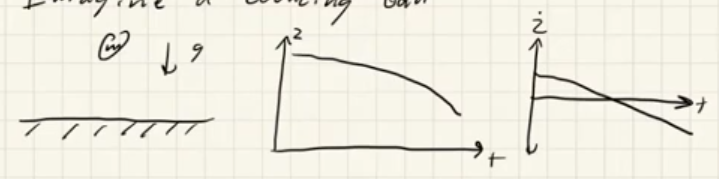
\includegraphics[width=0.4\linewidth]{L12_Images/F2.PNG}
    \caption{Bouncing ball}
    \label{fig:l12f2}
\end{figure}
\begin{figure}
    \centering
    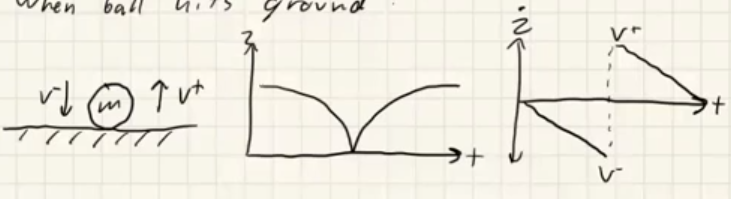
\includegraphics[width=0.4\linewidth]{L12_Images/F3.PNG}
    \caption{Hits ground}
    \label{fig:l12f3}
\end{figure}
\begin{itemize}
    \item Imagine a bouncing ball.
    \item In the air, dynamics are described by smooth ODE ($ m \ddot z = -g $)
    \item When ball hits ground:
    \item Because of the discontinuities, can't write down dynamics around impact as an ODE.
\end{itemize}

\subsubsection{Two Options:}
1) Event-based/hybrid formulation: Integrate ODE while checking for contact events using a "guard function" (e.g. $z \geq 0$). When contact event happens, execute "jump map" that models discontinuity, then continue integrating ODE. \\
2) Time-Stepping / Contact-implicit formulation: Solve a constrained optimization problem at every time step that enforces no interpenetration between objects ($\phi(x) \geq 0$) by solving for contact forces (HW 1 brick problem).

\begin{itemize}
    \item Both are widely used in simulation and have pros/cons.
    \item In control, hybrid formulation is easy to apply with standard algorithms (e.g. DDP/DIRCOL) and is most common.
    \item Downside: requires pre-specified contact mode sequence (which part of the robot is in contact at each time step).
    \item Despite this, hybrid methods have been very successful in locomotion.
    \item Contact-implicit method doesn't need mode sequence pre-specified but the optiimization problems are much harder. Active research area.
\end{itemize}





